\documentclass{acm_proc_article-sp}
\usepackage[utf8]{inputenc}
\usepackage{url}
\usepackage{listings}
\usepackage{color}
\usepackage{graphicx}
\graphicspath{{./imagens/}}

 
\definecolor{dkgreen}{rgb}{0,0.6,0}
\definecolor{gray}{rgb}{0.5,0.5,0.5}
\definecolor{mauve}{rgb}{0.58,0,0.82}
\definecolor{dkblue}{rgb}{0,0,.6}
\definecolor{dkyellow}{cmyk}{0,0,.8,.3}

\begin{document}

\title{Construindo Web Services Utilizando SOAP}
%\titlenote{(Does NOT produce the permission block, copyright information nor page numbering). For use with ACM\_PROC\_ARTICLE-SP.CLS. Supported by ACM.}}
%\subtitle{[Extended Abstract]
%\titlenote{A full version of this paper is available as
%\textit{Author's Guide to Preparing ACM SIG Proceedings Using
%\LaTeX$2_\epsilon$\ and BibTeX} at
%\texttt{www.acm.org/eaddress.htm}}}

\numberofauthors{5} 

\author{
	\alignauthor
	Juliano Rodovalho\\
		   \affaddr{Fedaral University of Pampa}\\
		   \affaddr{Av Tiarajú, 810}\\
		   \affaddr{Alegrete - RS}\\
		   \email{j.rodovalho.m@gmail.com}
	% 2nd. author
	\alignauthor
	Rafael T. Amorim\\
		   \affaddr{Fedaral University of Pampa}\\
		   \affaddr{Av Tiarajú, 810}\\
		   \affaddr{Alegrete - RS}\\
		   \email{jrtadf@gmail.com}
	% 3rd. author
	\alignauthor  Renan M. Uchôa\\
		   \affaddr{Fedaral University of Pampa}\\
		   \affaddr{Av Tiarajú, 810}\\
		   \affaddr{Alegrete - RS}\\
		   \email{renanmarceluchoa@gmail.com}
	\and  % use '\and' if you need 'another row' of author names
	% 4th. author
	\alignauthor Helison R. Teixeira\\
		   \affaddr{Fedaral University of Pampa}\\
		   \affaddr{Av Tiarajú, 810}\\
		   \affaddr{Alegrete - RS}\\
		   \email{helisonreus@gmail.com}
	% 5th. author
	\alignauthor Lucas P. Capanelli\\
		   \affaddr{Fedaral University of Pampa}\\
		   \affaddr{Av Tiarajú, 810}\\
		   \affaddr{Alegrete - RS}\\
		   \email{lucas.capanelli.es@gmail.com}
%	\alignauthor 
}


\maketitle
\begin{abstract}

		Esse artigo tem como objetivo mostrar uma visão geral sobre \emph{Web Services}, demonstrando o funcionamento de um \emph{Web Services} criado em PHP utilizando o \emph{Zend Framework} e o protocolo SOAP, para isso é dada uma explicação inicial de como funciona um \emph{Web Services}, de sua arquitetura e principais características, em seguida é exibido um exemplo de um \emph{Web Services}, o que é necessário ser feito para que o mesmo funcione corretamente.
		
		
		\emph{This article is intended to show an overview about webservices tecnologies, showing how stuff works a SOAP Web services in PHP with Zend Framework, for that are given an initial explanation of how \emph{Web} services works, the architeture and their main features, then is established a example of  \emph{Web} services, what must be done for it works properly.}
			
\end{abstract}

\keywords{Webservices, SOAP, XML} 

\section{Introdução}

		\emph{Web Services} trouxeram uma nova forma de construir Sistema Distribuídos, e com a \emph{Service Oriented Architeture} (SOA), uma nova filosofia de integrar sistemas e serviços. Mas para compreender como os \emph{Web Services} se comportam, é preciso dominar, antes de tudo, um pouco sobre o \emph{Service Oriented Architeture Protocol} (SOAP) que ele implementa, a tecnologia \emph{Extensible Markup Language} (XML) que é utilizada pelo protocolo para trafegar as mensagens entre os processos, e o próprio \emph{Hypertext Transfer Protocol} (HTTP) que é utilizado para encapsular o protocolo SOAP de comunicação durante as requisições cliente-servidor.
		
\section{Base Tecnológica}
		
	\subsection{XML}
	
		XML é uma linguagem de marcação extensível, projetada para transportar, armazenar e processar dados. O XML representa um conjunto de especificações especificadas e relatadas pelo \emph{World Wide Web Consortium}(W3C) e outros. O XML possui um ancestral em comum com o \emph{Standard Generalized Markup Language}(SGML). Uma das características do SGML era a separação do formato do conteúdo. Se um documento foi produzido para o formato A4 ou carta, por exemplo, o formato era descrito independentemente do conteúdo do documento. O mesmo documento portanto pode ser enviado em vários formatos sem mudar seu conteúdo. O principio das linguagens de marcação são aplicadas para os \emph{Web Services} através da separação da instancia do documento, que contém os dados, e o esquema, que descreve a estrutura dos dados e os tipos, incluindo informações de semântica muito úteis para fazer o mapeamento do documento para várias linguagens de programação e sistemas de software.
		
		O XML é similar ao \emph{HyperText Markup Language}(HTML), contém elementos, atributos e valores. Bem feitos os documentos em XML podem ser exibidos em navegadores \emph{Web}, porém, esse aspecto do XML não é muito relevante para os \emph{Web Services}. O HTML contém um conjunto finito de elementos e atributos, porém o XML permite ser definido tantos conjuntos quanto necessários.
		
		Os elementos e atributos de um arquivo XML definem independentemente seus tipos e estruturas de informação para o tipo de dado que eles contém, incluindo a capacidade de modelar dados e estruturas especificas à um domínio de \emph{software}. (Um domínio de \emph{software} pode ser uma linguagem de programação, um \emph{middleware}, um pacote de aplicações, ou um sistema de gerenciamento de dados). A transformação de uma representação genérica de dados contida em um XML em aplicativo, ou domínio de \emph{software}. A representação específica de dados é o aspecto principal dos \emph{Web Services}.\cite{UNDERWEBSERVICES}
		

	\subsection{HTTP}
	
		Em 1989, enquanto trabalhava no \emph{CERN}, Tim Berners-Lee teve a ideia que permitiria que os documentos na 
		internet pudessem acessar um ao outro. Em termos básicos, um documento poderia conter links que
		levassem a outros documentos, incluindo um texto especifico dentro dos documentos. A língua usada
		para criar esses documentos era a \emph{Hipertext Markup Language}(HTML). Em 1990, a internet nasceu com
		o primeiro documento HTML na internet. O HTML é baseado no SGML com algumas funcionalidades adicionais, como os hiperlinks
		e ancoras. Especificamente criado para a internet, o HTML apresentou um pequeno conjunto de tags que foram projetadas
		para exibir conteúdo, fazendo com que a adoção do HTML se espalhasse muito rapidamente.\cite{PRO_PHPXML}
	
		O HTTP é um protocolo de nível de aplicação, utilizado em sistemas distribuídos, colaborativos e sistemas de informação multimídia. É um protocolo genérico, e não proprietário pode ser usado para muitos objetivos, além do hipertexto, como domínios de servidores e gerenciamento de objetos de sistemas distribuídos, através da extensão de seus métodos de requisição, códigos de erro e cabeçalhos. Uma característica do HTTP é a escrita e negociação da representação de dados, habilitando os sistemas a fazer a construção dos dados a serem transferidos independentemente.\cite{HTTP-1.1}
	

	\subsection{SOAP}
	
		\subsubsection{O que é?}
	
			\emph{Simple Object Access Protocol} ou protocolo simples de acesso a objetos, conhecido como SOAP, é um protocolo de \emph{Web Services} que utiliza o formato XML para troca de mensagens. O padrão do protocolo SOAP é reconhecido pela W3C desde 2003 em sua versão 1.2. Inicialmente tendo a empresa de tecnologia \emph{Microsoft} como seu maior apoiador, no entanto é governado pela W3C atualmente.
		
			O SOAP é orientado a métodos, estes métodos podem ter ou não parâmetros, portanto é necessário o conhecimento da assinatura dos métodos. A execução dos métodos é realizada no servidor.
		
			Existem duas versões do SOAP: 1.1 e 1.2. Dentre as diferenças, pode-se mencionar que a versão 1.1 suporta apenas o HTTP com transporte de mensagens, enquanto a versão 1.2 permite a utilização de outros protocolos de transporte além do HTTP. \cite{WEBSERVICESZEND}
		
		\subsubsection{Funcionamento}
		
			Para descrever um \emph{Web Services} é utilizado vocabulário em XML chamado \emph{Web Service Description Language} conhecido como WSDL, que define como o \emph{Web Services} é acessado, quais as operações existem, como as mensagens são transferidas e a estrutura das mensagens. O WDSL não é obrigatório para trabalhar com \emph{Web Services}, ele faz uma parte integral do perfil do básico WS-I da organização \emph{OASIS Web Services Interoperability} \footnote{A \emph{Web Services Interoperability Organization} (WS-I) é uma organização aberta com objetivo de estabelecer as melhores práticas para a interoperabilidade de \emph{Web Services}, para grupos selecionados de padrões de \emph{Web Services}, através de plataformas, sistemas operacionais e linguagens de programação.\cite{OASIS-WS-I-SITE}} e facilita o trabalho.
			
			Através do WSDL, podemos saber quais métodos e parâmetros devemos enviar na requisição em XML. A especificação SOAP define um framework de mensagens para troca de XML formatado pela Internet.
			
			%
			%
			% RENAN !!!!!!!!!!!! FAZER ESTRUTURA DO XML SOAP !!!!!!
			%
			%
		
		
	\subsection{WSDL}
		
		O \emph{Web Services Description Languages} (WSDL) foi desenvolvido pela IBM em conjunto com a \emph{Ariba} e a \emph{Microsoft}, o WSDL é uma linguagem baseada em XML que proporciona um modelo para descrição de \emph{Web Services}. O padrão define serviços como portas ou \emph{endpoints }de redes. WSDL é usada normalmente em conjunto com o SOAP e esquemas em XML, para proporcionar o funcionamento de \emph{Web Services} através das redes. Uma aplicação que se conecta ao \emph{Web Services} para fazer uma requisição de serviço pode ler o WSDL para determinar quais funções estão disponíveis no \emph{Web Services}. Tipos de dados especiais são incorporados ao arquivo WSDL em forma de um esquema XML. O cliente pode então usar o SOAP para chamar funções listadas no WSDL.
		
		Por padrão é habilitada uma especificação para separar a descrição da funcionalidade abstrata oferecida pelo \emph{Web Services} dos detalhes concretos de uma descrição de serviço onde aquela funcionalidade é oferecida. Essa especificação define a linguagem para descrever a funcionalidade abstrata de um serviço bem como um \emph{textframework} para descrever os detalhes concretos da descrição de um serviço. A definição abstrata das portas e mensagens são separadas dos seus usos concretos, habilitando o reuso dessas definições. Uma porta é definida associando um endereço de rede com uma ligação reutilizável e uma coleção de portas define um serviço. As mensagens são descrições abstratas dos dados sendo trocados e tipos de portas são coleções abstratas de operações suportadas. O protocolo concreto e especificações dos formatos dos dados para um tipo de porta em particular constituem uma ligação reutilizável onde as mensagens e as operações são então ligadas a um protocolo de rede e um formato de mensagem concreta. \cite{APACHE-AXIS}
		
		
	\subsection{SOA}
		
		São políticas, práticas e estruturas que permitem que funcionalidades de um aplicativo seja prestado e consumido como conjuntos de serviços publicados, que podem ser invocados, publicado e descoberto, e são abstraídos da implementação usando um único modelo com base em um padrões de interface.\cite{SOA-Microsoft}
		
		Um sistema distribuído é composto de diversos agentes de software, discretos que devem trabalhar em conjunto para executar algumas tarefas. Além disso, os agentes em um sistema distribuído não operam no mesmo ambiente de processamento, por isso eles devem se comunicar por pilhas de de protocolo de hardware/software em uma rede. Isto significa que as comunicações com um sistema distribuído são intrinsecamente menos rápidas e confiáveis do que aqueles que usam invocação direta de código e memória compartilhada. Isto tem importantes implicações arquitetônicas porque sistemas distribuídos exigem que os desenvolvedores (da infra-estrutura e aplicações) considerem a latência imprevisível do acesso remoto, e levem em conta as questões de concorrência e da possibilidade de fracasso parcial.
		
		Uma Arquitetura Orientada a Serviços (SOA) é uma forma de arquitetar sistemas distribuídos caracterizada pela granularidade, visão lógica, plataforma neutra, orientação a mensagens, orientação a descrição, orientação pela rede.\cite{SOA-W3C}
		
		Na verdade os serviços da Web não são um componente obrigatório de uma SOA, embora cada vez mais eles venham se tornar desta maneira. SOA é potencialmente muito mais amplo em seu escopo do que simplesmente definir a implementação do serviço, abordando a qualidade do serviço a partir da perspectiva do fornecedor e do consumidor. Você pode fazer um paralelo com a CBD e tecnologias de componentes. COM e componentes UML da embalando componentes de endereço a partir do ponto de vista tecnológico, mas CBD, ou mesmo Componentes Baseados em Engenharia de Software (CBSE), é a disciplina com que você garante que está criando componentes que estão alinhados com o negócio. Da mesma forma, os \emph{Web Services} são puramente a implementação. SOA é a abordagem, não apenas o equivalente a serviço de um diagrama da embalagem do componente UML.\cite{SOA-Microsoft}
		
	\subsection{Web Services}
		
		\emph{Web Services} são formas de utilizar XML para mapear programas, objetos ou banco de dados ou para funções de negócio abrangentes. Usando um documento XML criado na forma de uma mensagem, um programa envia uma requisição para um \emph{Web Services} através da rede, e eventualmente recebe uma resposta também na forma de um documento XML. Os padrões do \emph{Web Service} definem o formato das mensagens, especificam a interface para qual as mensagens são enviadas, descrevem as convenções para mapear os conteúdos das mensagens dentro e fora dos programas que implementam o serviço, e definem mecanismos para publicar e para descobrir interfaces de \emph{Web Services}.
		
		\emph{Web Services} oferecem uma camada de abstração acima dos sistemas existentes, assim como Servidores de Aplicação, \emph{CORBA}, servidores \emph{.Net}, aplicativos mensageiros e pacotes de aplicação. \emph{Web Services} trabalham sobre 
		uma camada de abstração similar a da Internet e são compatíveis de realizar a transição entre qualquer sistema operacional, plataforma de hardware ou linguagem de programação, assim como a WEB é.
		
		Ao contrário dos sistemas distribuídos existentes, os \emph{Web Services} são adaptados para a \emph{Web}. A maioria das tecnologias de computação distribuída incluem os protocolos de comunicação em seu escopo. Com \emph{Web Services} os protocolos de comunicação já estão prontos e disponíveis por toda a \emph{Web}. 
		
		Esta tecnologia pode ser usada de várias maneiras. \emph{Web Services} podem ser executados em clientes de \emph{desktop} e portáteis para acessar aplicações de Internet, tais como sistemas de reservas e sistemas de controle de pedidos. \emph{Web Services} também podem ser usados para integração \emph{business-to-business} (B2B), conectando aplicativos executados por diversas organizações na mesma cadeia de fornecimento. \emph{Web Services} podem também resolver um dos problema mais amplo de integração de aplicações empresariais (IAE), conectando múltiplas aplicações de uma única organização a vários outros aplicativos, tanto dentro como fora do \emph{firewall}. Em todos estes casos, as tecnologias de \emph{Web Services} fornecem o padrão que liga diversas peças de software.\cite{UNDERWEBSERVICES}
		
		\subsubsection{O que são?}
		
			\emph{Web Services} é um método de comunicação entre dispositivos computacionais distribuídos pela \emph{World Wide Web}(Web), um \emph{Web Services} pode converter sua aplicação em uma aplicação \emph{Web} que poderá publicar suas funções ou mensagens para o restante da WEB, sua arquitetura consiste em oferecer arquivos XML contendo as informações requisitadas por seus clientes, de acordo com sua game de conteúdos disponíveis.\cite{WEBS}
		
		\subsubsection{Funcionamento}
		
			\emph{Web Services} normalmente são implementados usando linguagens de programação projetados para interação com a \emph{Web}, como \emph{Java Servlets} ou \emph{Application Server Pages} (ASPs) que exigem um programa de \emph{back-end}.
			
			Como visto na Figura \ref{fig:WebServiceFuncionamento}, para um programa submeter um documento para o \emph{Web Service} ele utiliza um esquema XML de um tipo específico, como o WSDL. Para transformar os dados de seu arquivo de origem nesse exemplo e produzir um documento XML no formato compatível com o que o \emph{Web Service} de destino espera, é descrito no mesmo arquivo WSDL. O arquivo WSDL é utilizado para definir a transformação dos dados de entrada e saída.
			
			\begin{figure}[h]
				\begin{center}
					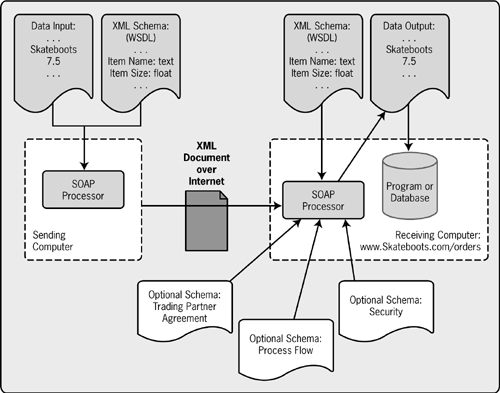
\includegraphics[width=250px]{WebServiceFuncionamento}
						\caption{Web Services use XML documents and transform them into and out of programs }
					\label{fig:WebServiceFuncionamento}
				\end{center}
			\end{figure}
			
			O SOAP do computador que esta enviando a mensagem transforma seus dados da forma nativa para o esquema XML pré-definido contido no arquivo WDSL para texto, pontos flutuantes, e outros, usando o mapeamento das tabelas. O Mapeamento das tabelas associa tipos de dados nativos com os tipos de dados correspondentes no XML. Padrões de mapeamento estão disponíveis para \emph{Java}, \emph{Visual Basic}, \emph{CORBA}, e outros tipos mais comuns de tipos de sistema. Muitas ferramentas XML estão disponíveis para definir mapeamentos customizados ou especiais. O computador que recebe o processo SOAP executa a transformação reversa, mapeando os tipos de dados do XML para os seus tipos de dados correspondentes.
			
			A sintaxe usada nas tecnologias de \emph{Web Services} especifica como os dados são genericamente representados, define como e com quais qualidades de serviço os dados são transmitidos, e detalha como o serviço é enviado e recebido. As implementações de \emph{Web Services} decodificam esses vários bits de XML para interagir com várias aplicações e domínios de software por baixo do serviço.
					
			
			A URL é amplamente utilizada na \emph{Web}, ela aponta para um endereço de TCP(\emph{Transmission Control Protocol}) que contém um recurso \emph{Web}. Os esquemas de \emph{Web Services} são formulários de recursos \emph{Web}, eles se encontram em arquivos acessíveis pela internet e publicados na \emph{Web} utilizando o mesmo mecanismo utilizado para downloads de arquivos via HTML. A grande diferença entre fazer downloads via HTML e o acesso de recursos do Web Service, é que os \emph{Web Services} utilizam o XML ao invés de documentos HTML e dependem das tecnologias associadas, como os esquemas, transformações e a validação para poder suportar remotamente a comunicação entre aplicações clientes e servidor. Mas a forma em que os esquemas \emph{Web Services} são publicados e baixados é a mesma: uma operação HTTP em uma determinada URL.\cite{UNDERWEBSERVICES}

			
		
\section{Implementação}

\lstset{ 
	language=php,               
	breaklines=true,                
	breakatwhitespace=false,        
	basicstyle      = \small\ttfamily,
	  keywordstyle    = \color{dkblue},
	  stringstyle     = \color{red},
	  identifierstyle = \color{dkgreen},
	  commentstyle    = \color{gray},
	  emph            =[1]{php},
	  emphstyle       =[1]\color{black},
	  emph            =[2]{if,and,or,else},
	  emphstyle       =[2]\color{dkyellow},
	  emph            =[3]{as,new,public,function,return,class,private,null,extends},
	  emphstyle       =[3]\color{dkblue},
	captionpos=b,
	numbers=left,                   % where to put the line-numbers
		numberstyle=\tiny\color{gray},  % the style that is used for the line-numbers
     stepnumber=1       
}

	Para a demonstração da implementação de um \emph{Web Services}, foi desenvolvida uma aplicação de agenda telefônica com servidor(\emph{Web Services}) em linguagem de programação PHP junto ao \emph{Zend Framework} e uma aplicação cliente para o sistema \emph{Android} desenvolvida com \emph{PhoneGap} e \emph{framework javascript JQuery Mobile}.
	
	\subsection{Aplicação Servidor}

	Para o desenvolvimento de um \emph{Web Services}, utilizamos uma classe do \emph{Zend Framework} chamada Zend\_Soap\_Server que fornece toda funcionalidade de um \emph{Web Services} no protocolo SOAP. 
	
	Na listing \ref{listing:CriacaoWebServices}, temos a instanciação da classe e a configuração do \emph{Web Services}, onde passamos um vetor com a versão do protocolo SOAP para 1.2, url do \emph{Web Services} e codificação de caracteres. Logo em seguida é informada a url do WSDL e a classe que possui os serviços que serão disponibilizados. E finalmente o método \emph{handle()} para inicializar o \emph{Web Services}.
	
	\lstinputlisting[language=PHP,caption={Criação de Web Services},label={listing:CriacaoWebServices}]{start_web_services_server.php}
	
	Para quem for usar o \emph{Web Services} saiba as operações que possam ser realizadas, utilizamos o WSDL para descrever os serviço da API em detalhes. Foi utilizado um componente do \emph{Zend Framework}, a classe Zend\_Soap\_AutoDiscover que permite detectar automaticamente e realizar o mapeamento do da classe de serviço. Na listing \ref{listing:GeracaoWSDL}, verificamos se existe algum pedido de WSDL por parâmetro \emph{GET}, caso exista ocorre a instanciação da classe \emph{AutoDiscover} que faz a leitura da classe de modelo por meio de \emph{reflection} e gera o mapeamento WSDL.
	
	\lstinputlisting[language=PHP,caption={Geração do WSDL},label={listing:GeracaoWSDL}]{web_services_wsdl.php}
	
	Na classe de serviço, foi adicionado as operações disponíveis do \emph{Web Services} para adicionar, remover e listar os contatos da agenda telefônica como mostrado na listing \ref{listing:ClasseServicos}.
	
	\lstinputlisting[language=PHP,caption={Classe de Serviços},label={listing:ClasseServicos}]{classe_servico.php}
	
	\subsection{Aplicação Cliente}
	
	No cliente, foi desenvolvida uma aplicação utilizando \emph{PhoneGap} e \emph{JQuery Mobile}. O PhoneGap permite o desenvolvimento de aplicações móveis para \emph{iOS, Android, Blackberry, Windows Phone, Palm WebOS, Bada} e \emph{Symbian} utilizando simplesmente: \emph{HTML, CSS} e \emph{Javascript}.\cite{PHONEGAPSITE}
	
	\emph{JQuery Mobile} fornece um sistema de interface unificado baseado em HTML5 para todas as populares plataformas.\cite{JQUERYMOBILESITE}
	
	Para realizar a comunicação com \emph{Web Services}, foi criada uma classe \emph{WebService} como na listing \ref{listing:ClasseClienteWebservice}, esta classe trata de realizar uma conexão HTTP e mandar o XML por \emph{POST}.
	
	\lstinputlisting[language=php,caption={Classe Cliente de Webservice},label={listing:ClasseClienteWebservice}]{classe_cliente.js}
	
	Na listing \ref{listing:TemplateSOAP}, temos os \emph{templates} em xml das operações que serão realizadas. A primeira operação insere um contato no \emph{Web Services}, onde temos a estrutura completa do SOAP envelope, cabeçalho e o corpo que contem a operação que estamos requisitando e os parâmetros.
	
	\lstinputlisting[language=html,caption={Templates SOAP},label={listing:TemplateSOAP}]{template_soap.html}
 
\section{Como Utilizar}

	\subsection{Requisitos}
	
	Para a execução da aplicação de demonstração, é necessário ter os seguintes requisitos cumpridos:
	
		\begin{itemize}
			\item Servidor Web com PHP 5.4 ou superior
			\item Eclipse IDE com plugin Android ADT
			\item Android SDK level 10 ou superior
		\end{itemize}
	
	Para a instalação do servidor web, é recomendado o projeto XAMPP que roda em sistemas Microsoft Windows, cujo link para download é: \url{ http://www.apachefriends.org/pt_br/xampp-windows.html}
	
	Para a utilização da aplicação web, é recomendado a instalação da \emph{IDE Eclipse}, cujo link para download é: \url{http://www.eclipse.org/downloads/packages/eclipse-ide-java-ee-developers/junor} e o plugin \emph{ADT} do \emph{Android} para o \emph{Eclipse}, cujo link para o tutorial de instalação e download é: \url{http://developer.android.com/sdk/installing/installing-adt.html}
		
	\subsection{Servidor}
	
		Para utilizar o servidor deve-se ter o servidor web instalado previamente e realizar o download do seguinte pacote e extrair na pasta htdocs do servidor, no caso do XAMPP localizado na C:\textbackslash xampp\textbackslash htdocs
	
		Código fonte do servidor: \url{https://github.com/rmuchoa/AgendaTelefonica/zipball/master}
		
		Logo em seguida, é necessário criar o banco de dados da aplicação servidor, navegue até o diretório da aplicação servidor e digite: 
		
			\emph{php script/setup-db.php}
		
		Após isto, o webservice poderá ser acessado pela url: \url{http://localhost/NomePastaProjeto/public/webservice.php}
	
	\subsection{Cliente}
	
		Para acessar o web service com a aplicação cliente, é necessário ter instalado o \emph{Eclipse} com plugin ADT e o SDK Android Level 10 ou superior. Baixe uma cópia do cliente na URL: \url{https://github.com/rmuchoa/AgendaTelefonica/zipball/android-app}

		Abra o eclipse e crie uma maquina virtual do Android na aba Window > ADV(Android Virtual Device) Manager, clique em New e preencha o nome, tamanho do cartão de memória e crie a ADV então irá aparecer na lista no manager, clique em Start, aguarde carregar o emulador. Em seguida, em projetos do eclipse, clique com botão direto no projeto: Run as > Android Application. 
		
		A aplicação cliente irá iniciar e pedir a URL do web service, informe a url \url{http://localhost/NomePastaProjeto/public/webservice.php}, substitua de acordo com localização da pasta do projeto e clique em OK.
	
		
	
\section{Conclusão}

	O \emph{Web Service} nos forneceu a interoperabilidade necessário entre sistemas distribuídos, a partir de suas operações foi possível realizar a comunicação entre aplicações construídas em diferentes plataformas e linguagens de programação, como neste artigo, onde utilizamos uma aplicação em PHP e outra em \emph{Javascript}, sendo o servidor e o cliente, respectivamente. 
	
	
 
\bibliographystyle{abbrv}
\bibliography{sigproc}  % sigproc.bib is the name of the Bibliography in this case

\end{document}
